% Active slide. \input by main.tex; variants via promote-slide.sh (-s 06-scalar -v <suffix>)
% --- 06 Scalar optimization (Zbc clmul) --------------------------------------
% Slide 1: word-level clmul concept (schoolbook -> word-level leaf).
% Slide 2: compile-time specialization (static generator + assign-on-first-write
%          + multi-backend), cumulative scalar polymul speedup.
% src (headline x101.3): results/reports/summaries/speedups_simulation.md,
%   Table 1 vect_mul, Spike instret, HQC-128: 18,504,302 -> 182,726 = x101.3.
% src (assign-on-first-write -21%): results/reports/ablation/
%   polymul_scalar_zbc.md, transition AC->ACB instret x1.27 (HQC-128).

\begin{frame}[fragile]{Tier 1: ο word-level \clmul αντικαθιστά τον bit-serial schoolbook}
  \vspace{0.5em}
  Ο εσωτερικός βρόχος των 64 \en{bits} \HL{εξαλείφεται} (64 \en{iterations} $\to$ 1)
  \vfill
  \begin{center}
    \adjustbox{max width=\linewidth,max totalheight=0.64\textheight,center}{% Comparison: bit-serial schoolbook vs word-level clmul leaf
% Used in §6.2.1 (ssec:bit-to-word)

\tikzsetnextfilename{ch6-polymul-schoolbook-vs-clmul}
\begin{tikzpicture}[
  box/.style={draw, rounded corners=2pt, minimum width=4.8cm,
    minimum height=2.2cm, align=left, font=\ttfamily\small},
  arrow/.style={->, thick, >=stealth},
  label/.style={font=\sffamily\small\bfseries, above}
]

% Left box: bit-serial schoolbook
\node[box, fill=red!5] (school) at (0,0) {%
  \begin{tabular}{@{}l@{}}
  for i in 0..n-1:\\
  \quad for bit in 0..63:\\
  \quad\quad mask = -(a[i]>>bit \& 1)\\
  \quad\quad for j in 0..n-1:\\
  \quad\quad\quad r[i+j] \^{}= (b[j]<<bit) \& mask\\
  \quad\quad\quad r[i+j+1] \^{}= (b[j]>>inv) \& mask
  \end{tabular}
};
\node[label] at (school.north) {Bit-serial schoolbook};
\node[font=\sffamily\footnotesize, below=2pt] at (school.south)
  {$64 \times n^2$ conditional shift-XOR};

% Right box: clmul leaf
\node[box, fill=green!5] (clmul) at (7.5,0) {%
  \begin{tabular}{@{}l@{}}
  for i in 0..n-1:\\
  \quad for j in 0..n-1 (pairs):\\
  \quad\quad lo = clmul(a[i], b[j])\\
  \quad\quad hi = clmulh(a[i], b[j])\\
  \quad\quad r[i+j] \^{}= lo\\
  \quad\quad r[i+j+1] \^{}= hi
  \end{tabular}
};
\node[label] at (clmul.north) {Word-level \textsf{Zbc} leaf};
\node[font=\sffamily\footnotesize, below=2pt] at (clmul.south)
  {$n^2$ ζεύγη clmul/clmulh};

% Arrow between
\draw[arrow, very thick, color=blue!60!black]
  (school.east) -- node[above, font=\sffamily\small] {$\times$64}
  (clmul.west);

\end{tikzpicture}
}
  \end{center}
  \vfill
\end{frame}

\begin{frame}[fragile]{Tier 1: \en{static code generator} + \en{assign-on-first-write}}
  \begin{itemize}
    \item \HL{\en{Static code generator}}: δέντρο Karatsuba ως \en{literals} για σταθερά $N \in \{277, 561, 901\}$, \pos{μηδέν \en{runtime checks}}
    \item \HL{Τρία \en{backends}} από έναν \en{generator} (\code{--mode} \code{zbc}/\code{rvv}/\code{zvbc})
  \end{itemize}
  \vspace{0.2em}
  \begin{center}
    \adjustbox{max width=0.82\linewidth,max totalheight=0.30\textheight,center}{% AP-2 Generator Pipeline diagram
% Used in §6.2.3 (ssec:ap2-generator)

\tikzsetnextfilename{ch6-polymul-ap2-pipeline}
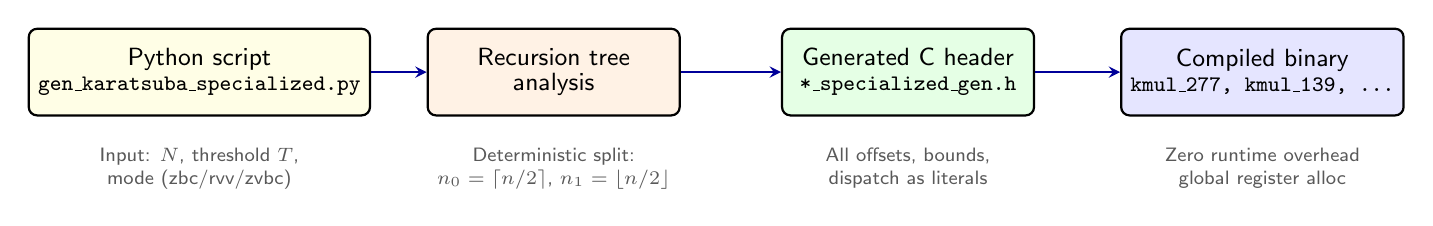
\begin{tikzpicture}[
  stage/.style={draw, rounded corners=3pt, minimum width=3.2cm,
    minimum height=1.1cm, align=center, font=\sffamily\small, thick},
  arrow/.style={->, thick, >=stealth, color=blue!60!black},
  note/.style={font=\sffamily\scriptsize, text=gray!70!black, align=center}
]

% Stage 1: Python script
\node[stage, fill=yellow!10] (script) at (0,0)
  {Python script\\[-2pt]\texttt{\footnotesize gen\_karatsuba\_specialized.py}};

% Stage 2: Recursion tree analysis
\node[stage, fill=orange!10] (tree) at (4.5,0)
  {Recursion tree\\[-2pt]analysis};

% Stage 3: Generated C header
\node[stage, fill=green!10] (header) at (9,0)
  {Generated C header\\[-2pt]\texttt{\footnotesize *\_specialized\_gen.h}};

% Stage 4: Compiled binary
\node[stage, fill=blue!10] (binary) at (13.5,0)
  {Compiled binary\\[-2pt]\texttt{\footnotesize kmul\_277, kmul\_139, \ldots}};

% Arrows
\draw[arrow] (script) -- (tree);
\draw[arrow] (tree) -- (header);
\draw[arrow] (header) -- (binary);

% Annotations below
\node[note, below=8pt] at (script.south) {Input: $N$, threshold $T$,\\mode (zbc/rvv/zvbc)};
\node[note, below=8pt] at (tree.south) {Deterministic split:\\$n_0 = \lceil n/2 \rceil$, $n_1 = \lfloor n/2 \rfloor$};
\node[note, below=8pt] at (header.south) {All offsets, bounds,\\dispatch as literals};
\node[note, below=8pt] at (binary.south) {Zero runtime overhead\\global register alloc};

\end{tikzpicture}
}
  \end{center}
  \vspace{0.2em}
  {\color{accent!40}\rule{\linewidth}{0.6pt}}
  \vspace{0.2em}
  \begin{itemize}
    \item \HL{\en{Assign-on-first-write}}: χωρίς μηδενισμό \en{buffer} ($0 \oplus x = x$), \con{$-\pct{21}$} \instret
  \end{itemize}
  \vspace{0.2em}
  \begin{block}{Αποτέλεσμα}
    Σωρευτικά \HL{\speedup{101.3}} σε \instret στον πυρήνα πολ/σμού \HQC-128.
  \end{block}
\end{frame}
